Dynamic Programming(DP) is unusually used in Optimization problem such as the first example. But it could be used in other field as well. In this example, DP is used in a counting problem.

Given a number of $m$ in unary, count the number $n$ of binary string of length $m$ that do not contain the pattern $11$. For instance, in the following example, there are $5$ strings with length $3$ which does not containing $11$. 

\begin{figure}[H]
	\centering
	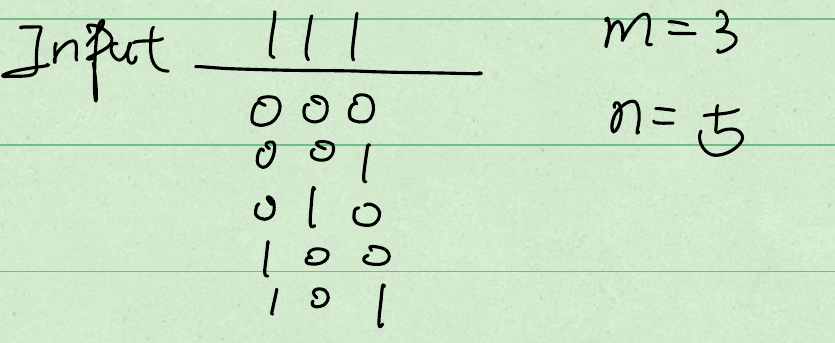
\includegraphics[width=0.3\textwidth]{fig/bin-pattern.png}
\end{figure}

\paragraph{Remark: why input is unary}The answer of the problem could be near $2^n$ string with $n$ bits long. If n is given by binary, your input is $\log n $ bits. In this case, even write down the answer would be an exponential time algorithm. Therefore, make the input unary reduce the size of the problem and make it solvable.

Say a string is valid if it does not contain the pattern ``$11$''.
\paragraph{Top Level Question:} 
\begin{itemize}
	\item Count the number of valid string of length $n$ ending in $0$.
	\item Count the number of valid string of length $n$ ending in $1$.
\end{itemize}

The valid strings of length $n$:
\begin{figure}[H]
	\centering
	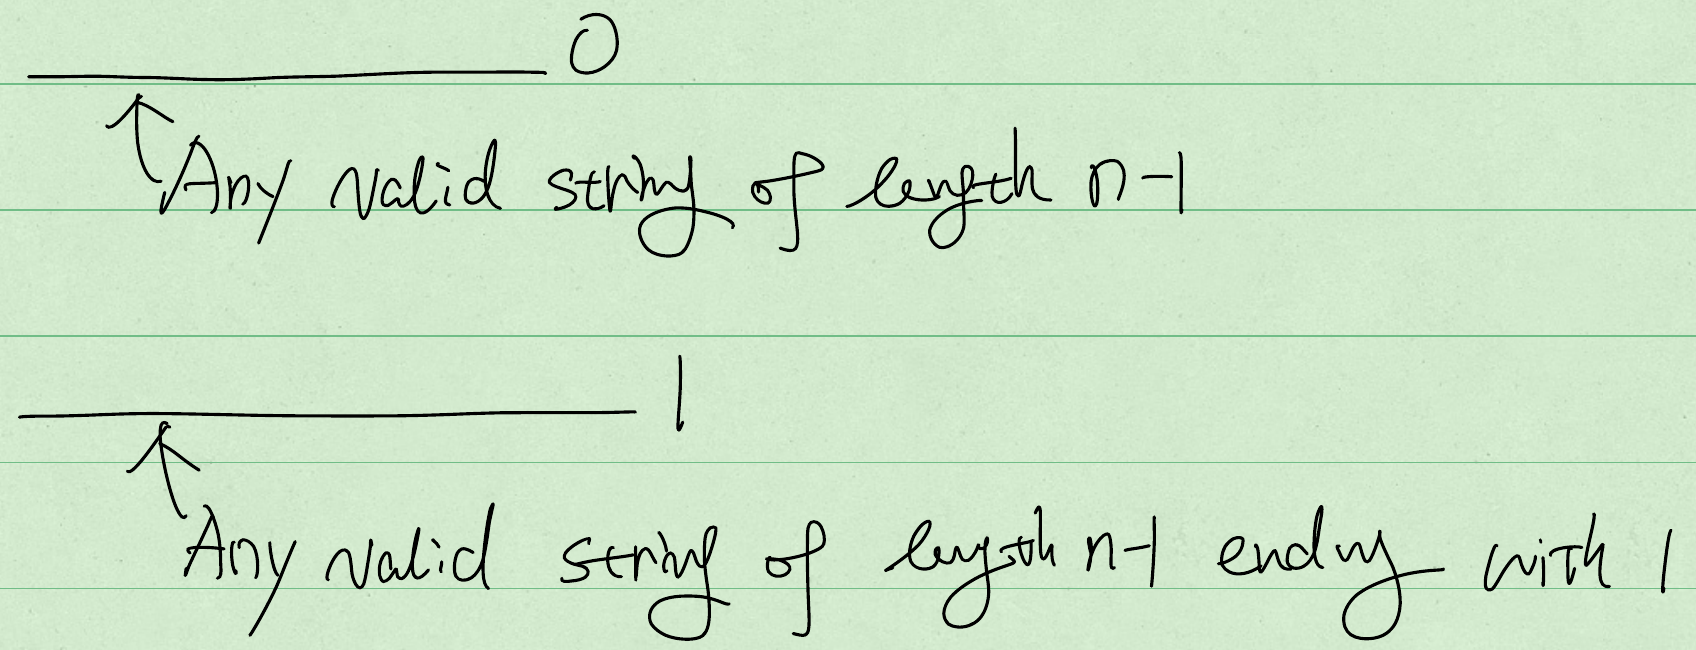
\includegraphics[width=0.5\textwidth]{fig/valid-str.png}
\end{figure}

Let make the following notation,
\begin{itemize}
	\item $S_1(n) = \#$ of valid string of length $n$, ending with $1$.
	\item $S_0(n) = \#$ of valid string of length $n$, ending with $0$.
\end{itemize}

So we have $S(n) = S_0(n) + S_1(n)$, where
\begin{align*}
	S_1(n) =& S_0(n-1)\\
	S_0(n) =& S(n-1) = S_0(n-1) + S(n-1) 
\end{align*}

Therefore, $S(n) = 2S_0(n - 1) + S_1(n - 1)$. In base cases, $S_1(1) = S_0(1) = 1$.

